The last decade was very fruitful in the field of subregular research.
New classes of subregular languages and mappings were uncovered for modeling natural language phenomena, and new learning algorithms were developed for these classes.
The subregular approach has been successfully applied to phonotactics \citep{Heinz10ldp}, rewrite processes in phonology and morphology \citep{Chandlee2014}, and even syntactic constraints over tree structures \citep{Graf18CLS}.
However, the rapid pace of the theoretical research has not been matched when it comes to engineering considerations.
Many of the proposed learning algorithms have not been implemented, and as a result, their performance on concrete data sets was not known.

My thesis is a first step towards closing this gap.
The development of my toolkit \emph{SigmaPie} has made it possible to evaluate subregular proposals over data sets of various degrees of abstractness.
The results in Chapters~ \ref{languageschapter} and \ref{mappingsschapter} show that this is a worthwile enterprise that yields new results that are relevant to computational and theoretical linguists.
Issues that may be negligible in theory become much more relevant when dealing with real-world data.
For instance, phonological features and natural classes are immaterial for claims about subregular complexity, nor do they affect learning under the idealized assumptions that are commonly made in the grammatical inference literature.
But when learning with realistic data, the inability to generalize across phonologically related sounds can cause the learner to fail unexpectedly, as was the case with the TSL learner \ref{TSLresultssection}.
This is a powerful demonstration of the importance of features and natural classes, two concepts for which linguists were advocating for decades.

That said, the work reported in this thesis is a starting point.
\emph{SigmaPie} and the experimental modeling approach I developed in this thesis could be taken in numerous directions to improve the balance between theory and practice in the subregular field.
In the last few pages of this thesis, I revisit the findings of the previous chapters, assess their implications for computational and theoretical linguistics, and outline potential future work. 
The latter might be the most important aspect of this thesis:
\emph{SigmaPie} provides a sandbox for tool-assisted subregular research, and there are many different things that can be done in this sandbox.
My thesis presented one particular use of \emph{SigmaPie}, but in order to unlock its full potential, the subregular community must keep adding new functionality to it and keep using it to probe the practical ramifications of its theorems and algorithms.



\section{Summary of the results}

My dissertation brings a two-sided approach to the problem of the theory-practice misbalance in subregular research.
First, I designed the Python package \emph{SigmaPie} \href{https://pypi.org/project/SigmaPie/}{\faCube}, which includes different subregular learners, scanners, sample generators, and some other functions that support subregular research \citep{sigmapie}.
Building on this package, I then explored the performance of several subregular learning algorithms on datasets that are modeled after widespread linguistic patterns such as word-final devoicing, harmonies of different types, and tone plateauing, among others.

\subsection{\emph{SigmaPie} \href{https://pypi.org/project/SigmaPie/}{\faCube}}

The package \emph{SigmaPie} mostly focuses on subregular languages and grammars, but also includes an implementation of \emph{OSTIA}, a learner for subsequential transducers \citep{OncinaEtAl1993,DeLaHiguera2010}.
The functionality of the package includes various functions that can be used to simplify the practical work with subregular languages.
\emph{Learners} extract subregular grammars from the provided dataset.
\emph{Scanners} evaluate the well-formedness of data items with respect to the given grammar.
\emph{Sample generators} produces a dataset of the required size that follows the given grammar.
\emph{Polarity switchers} convert the grammars from positive to negative, and the other way around.
Finally, \emph{FSM constructors} build a finite state machine based on the given grammar.
The implemented learning algorithms for strictly piecewise, strictly local, tier-based strictly local, and multi-tier strictly local languages are proposed in \citep{Heinz-2010-SEL,JardineMcMullin2017,McMullinAksenovaDeSanto2019}.
All of these aspects of \emph{SigmaPie} played a key role in the design of the experiments for this thesis.

\emph{SigmaPie} is implemented in Python 3, and uses the copyleft open-source \href{https://www.gnu.org/licenses/gpl-3.0.en.html}{GNU General Public License v3.0}.
It is available on PyPI and in \texttt{pip}.
\emph{SigmaPie} is an ongoing project and, by design, cannot be feature-complete as long as new subregular research keeps being published.
Researchers who modify or extend the code for their own projects are highly encouraged to create a pull request in the GitHub repository so that their code can be incorporated into future releases.


\subsection{Tool-assisted learning experiments: overview}

Building on the functionality provided by \emph{SigmaPie}, this dissertation also presented several learning experiments in Chapters~ \ref{languageschapter} and \ref{mappingsschapter}.
I used several wordlists from natural languages (Finnish, German, Turkish), and I also constructed artificial datasets exhibiting different linguistic patterns, e.g.\ word-final devoicing.
I then used \emph{SigmaPie} to test whether subregular learning algorithms can extract suitable grammars from these datasets.
The experiments conducted were of two types: the first type probed the learning of well-formedness conditions, while the second one explored generalizing the rules of rewrite processes.

The experiments on well-formedness conditions all follow the same procedure.
The input consists of lists of words that obey a specific well-formedness condition.
For example, if the condition to be tested is vowel harmony, then the training data includes only forms where all vowels agreed in the relevant harmony feature.
Alternatively, in the case of the word-final obstruent devoicing, the dataset only includes words that do not end in a voiced obstruent.
One of \emph{SigmaPie}'s learning algorithms is then used to infer a grammar from the dataset.
This grammar is then fed into \emph{SigmaPie}'s sample generator to produce a set of strings that are well-formed according to the learned grammar.
Finally, one of \emph{SigmaPie}'s scanner implementations is used to determine how many of these strings are well-formed with respect to the original grammar.
This generate-and-test paradigm is repeated multiple times to calculate an average accuracy score for the learner.

The learning of rewrite rules by the OSTIA algorithm follows a similar paradigm but changes some technical details.
Each training sample now consists of pairs of strings, which encode the underlying representation (UR) and the corresponding surface form (SF) that is produced by some rewrite rule.
As a toy example, assume that the inventory of vowels only contains $a$ and $o$, and that we have a progressive vowel harmony process that requires all vowels to agree in rounding.
Valid SFs then include either only $o$ vowels or only $a$ vowels.
The corresponding URs have all the non-initial vowels hidden (for example, represented as $A$), and only the initial vowel is specified as $a$ or $o$ to trigger the agreement.
%\footnote{
% In the encoding scheme used, the number of representations of vowels in the URs depends on the number of features that are important for the behavior of the vowels regarding the harmony.
% Namely, the number of vowel representations in URs is $2^f$, where $f$ is the number of such features.
% For example, in the mentioned toy pattern, no features were significant, and therefore there is only $2^0 = 1$ underspecified vowel.
% In some patterns, such as Turkish (see section 4.2.7), height plays a role in the behavior of the undergoers, and therefore there are $2^1 = 2$ underspecified vowels.
%}
In such a way, these pairs encode the URs that contain the underspecified elements, and the SFs where those elements are specified.

Note that the training data can exhibit various degrees of abstractness.
Consider the case of word-final obstruent devoicing in German, analyzed as a well-formedness condition rather than a rewrite rule.
A realistic dataset would be a finite list of attested German words.
A highly abstracted representation, on the other hand, would replace each German word with a string of $a$s and $b$s such that $a$ represents a voiced obstruent and $b$ any sound that is not a voiced obstruent.
One important insight of the experiments conducted in Chapter~\ref{languageschapter} is that the performance of a learning algorithm is not always uniform across these different levels of abstractness.
That is because a more abstract representation allows for fewer combinatorial possibilities --- with $k$ symbols, there are $k^n$ distinct $n$-grams, so the larger the value of $k$, the more $n$-grams there are.
The larger the space of combinatorial options, the more likely it is that the training data will miss a combination. 
Some subregular learners can easily get led astray by missing combinations, e.g.~the TSL learner, and as a result these learners fail to learn some phenomena over realistic data even if they succeed with the highly abstracted data sample.
Intuitively, this shows the importance of phonological features and natural classes, which allow the learner to generalize from observed combinations of sounds to other combinations that are missing in the data set.

The results of the learning experiments are summarized in Figure \ref{thesisresults}.
According to \cite{DeLaHiguera2010}, the task of grammatical inference algorithms is to \emph{constantly} predict the next correct element.
Therefore, an algorithm has not fully learned a pattern as long as it is still making errors, no matter how negligible or rare those errors are.
A single mistake means that the algorithm has failed to learn, and successful learning means perfect learning without any mistakes.
For this reason, Figure \ref{thesisresults} provides an abridged overview of the full results that were summarized in Figures \ref{languagesresults} and \ref{ostiaresults}.
% fixme: include page references (after the rest is ready)
In this abridged format, a success (\faThumbsOUp) indicates that the learner achieved an accuracy of $100\%$, and anything less than that is represented as a failure (\faTimes).

\begin{table}[h!]
\centering
\resizebox{\linewidth}{!}{%
\begin{tabular}{|l|c|c|c|c|c|}
\hline
\multicolumn{1}{|c|}{\multirow{2}{*}{\textbf{Experiments}}} &
\multicolumn{4}{|c|}{\textbf{Well-formedness}} &
\multicolumn{1}{|c|}{\textbf{Transformations}} \\ \cline{2-6} 

& \textbf{SP} & \textbf{SL} & \textbf{TSL} & \textbf{MTSL} & \textbf{OSTIA} \\ \hline

\textit{\textbf{E1:} word-final devoicing} 
& \cellcolor{gray!50}\faTimes
& \faThumbsOUp
&  \faThumbsOUp
& \faThumbsOUp
& \faThumbsOUp
\\ \hdashline

\textit{\textcolor{white}{\textbf{E1:}} learning from raw German data} 
& \cellcolor{gray!50}\faTimes
&  \faThumbsOUp
&  \faThumbsOUp
&\faThumbsOUp
& \cellcolor{black}
\\ \hline

\textit{\textbf{E2:} a single vowel harmony without blocking}
&           \faThumbsOUp     
& \cellcolor{gray!50}\faTimes
&  \faThumbsOUp
&\faThumbsOUp
& \faThumbsOUp
\\  \hdashline

\textit{\textcolor{white}{\textbf{E2:}} learning from raw Finnish data} 
&              \faThumbsOUp    
&        \cellcolor{gray!50}\faTimes
&  \cellcolor{gray!50}\faTimes
& \faThumbsOUp
& \cellcolor{black}
\\ \hline

\textit{\textbf{E3:} a single vowel harmony with blocking}           
& \cellcolor{gray!50}\faTimes
& \cellcolor{gray!50}\faTimes
& \faThumbsOUp
&\faThumbsOUp
& \cellcolor{gray!50}\faTimes
\\ \hline

\textit{\textbf{E4:} several vowel harmonies without blocking}       
& \faThumbsOUp
& \cellcolor{gray!50}\faTimes
& \faThumbsOUp
& \faThumbsOUp
&  \faThumbsOUp
\\ \hline

\textit{\textbf{E5:} several vowel harmonies with blocking}          
&         \cellcolor{gray!50}\faTimes      
& \cellcolor{gray!50}\faTimes
& \faThumbsOUp
&   \faThumbsOUp
&\cellcolor{gray!50}\faTimes
\\ \hdashline


\textit{\textcolor{white}{\textbf{E5:}} learning from raw Turkish data} 
&            \cellcolor{gray!50}\faTimes      
&        \cellcolor{gray!50}\faTimes
&  \cellcolor{gray!50}\faTimes
&\cellcolor{gray!50}\faTimes
& \cellcolor{black}
\\ \hline

\textit{\textbf{E6:} vowel and consonant harmonies without blocking} 
& \faThumbsOUp
& \cellcolor{gray!50}\faTimes
& \cellcolor{gray!50}\faTimes
& \faThumbsOUp
& \faThumbsOUp
\\ \hline

\textit{\textbf{E7:} vowel and consonant harmonies with blocking}    
& \cellcolor{gray!50}\faTimes
& \cellcolor{gray!50}\faTimes
& \cellcolor{gray!50}\faTimes
& \faThumbsOUp
&\cellcolor{gray!50}\faTimes
\\ \hline

\textit{\textbf{E8:} unbounded tone plateauing}                      
& \faThumbsOUp
& \cellcolor{gray!50}\faTimes
& \cellcolor{gray!50}\faTimes
& \cellcolor{black} 
& \cellcolor{gray!50}\faTimes
\\ \hline

\textit{\textbf{E9:} ``simple'' first-last harmony}                            
& \cellcolor{gray!50}\faTimes
& \cellcolor{gray!50}\faTimes
& \cellcolor{gray!50}\faTimes
& \cellcolor{gray!50}\faTimes
& \faThumbsOUp
\\ \hline

\textit{\textbf{E10:} ``complex'' first-last harmony}                            
& \cellcolor{black} 
& \cellcolor{black} 
&  \cellcolor{black} 
& \cellcolor{black} 
&\cellcolor{gray!50}\faTimes
\\ \hline
\end{tabular}}
\caption{Learning results that were experimentally obtained in this dissertation.
Black cells indicate that the experiments were not conducted due to the reasons discussed in \ref{omittedexpsection}.}
\label{thesisresults}
\end{table}

While these results largely mirror the theoretical expectations, they do not tell the full story.
The experiments for well-formedness conditions as well as the experiments for rewrite rules reveal subtle nuances of the subregular learning approach that deserve closer attention.

\subsection{Learning well-formedness conditions}
The learning of well-formedness conditions focused on four important subregular classes: strictly piecewise (SP), strictly local (SL), tier-based strictly local (TSL), and multi-tier strictly local (MTSL) languages.

SP grammars encode long-distance dependencies that prohibit certain substructures, while the distance between the elements of that substructure, as well as the type of intervening material, plays no role \citep{HeinzRogers2010SPdist,Heinz-2010-SEL}.
As a result, SP grammars are ideally suited to long-distance patterns as long as they do not involve blocking.
This is reflected in the training data.
The SP model achieved an accuracy of $100\%$ on all harmonies that do not exhibit a blocking effect, including the pattern of Finnish harmony learned from raw Finnish data, and even unbounded tone plateauing, which is challenge for other classes such as TSL and MTSL\@.
But the SP learner failed consistently on local processes such as word-final devoicing, and on long-distance processes that involve blocking.
Overall, then, the SP learning results are in line with the theoretical expectations.

At the same time, though, the SP learner performed unexpectedly well on some processes it should have failed on.
Most notably, it achieved an accuracy of 89\% on word-final devoicing.
But this should not be construed as a surprising ability of SP grammars to handle local processes over realistic data samples.
Thanks to the transparent nature of subregular grammars and learners, we could inspect the learned grammar and see that it does not enforce any kind of word-final devoicing.
The high accuracy score is an artefact that arises from the fact that it is very unlikely for a randomly generated string to have any obstruent at the end.
If we limited our attention to only strings that end in an obstruent, the performance of the learned SP grammar would be abysmal.
We see, then, that accuracy scores can be misleading when considered in a vacuum, and the linguistic transparency of the subregular approach allows us to reliably identify cases where the quantitative results do not match the qualitative facts.

The other classes SL, TSL, and MTSL also provide some interesting insights.
SL models only local phenomena and cannot handle long-distance dependencies.
This is reflected by learning results, where the SL learner succeeded only on word-final devoicing, but did so uniformly on all data sets, whether they were realistic or highly abstracted.
With SL learning, the previously mentioned issues of combinatorial explosion and data sparsity are much less relevant, at least as long as the $n$-grams are short.

A TSL grammar captures a single long-distance dependency \citep{HeinzRawal11,JardineMcMullin2017}.
In contrast to SP, it can handle blocking effects, but it fails on some long-distance phenomena such as unbounded tone plateauing.
Moreover, if different agreements affect different sets of elements, such as in the case of independent vowel and consonant harmonies, one needs several tiers.
This marks the step from TSL to MTSL.
Again the learning results largely match theoretical expectations \citep{DeSantoGraf19FG,McMullinAksenovaDeSanto2019}, with two notable exceptions.
The first one is the failure of the TSL algorithm to learn some phenomena over realistic data sets even though the algorithm succeeds over the abstracted dataset.
As explained earlier, this is a problem of combinatorial explosion: the TSL algorithm assumes that missing combinations always convey meaningful information about which sounds do or do not matter for the dependency, and as a result it is easily led astray by accidental gaps in the data.
The second unexpected result pertains to the MTSL learner.
This algorithm sometimes produced unnaturally large grammars with hundreds of tiers while a standard linguistic analysis would only posit a handful of tiers.
It is only because of the transparency of subregular methods that this shortcoming could even be noticed --- if the learners and grammars were opaque to human inspection, MTSL would seem to turn in a stellar performance across the board.
By looking under the hood, we see that the quantitative performance conceals some qualitative shortcomings, the cause of which will have to be left to future research.

Finally, none of the learners captured the unattested pattern of first-last harmony.
This is again in line with the theoretical predictions as first-last harmony does not fit into any of the classes SP, SL, TSL, or MTSL\@.
In sum, the finding of the learning experiments for well-formedness conditions can be summarized in the form of three key insights:

\begin{enumerate}
    \item \textbf{Theoretical predictions borne out}\\
          When trained on abstracted, artificially generated data, the subregular learners performed exactly as predicted by the theoretical work on subregular learning.
    \item \textbf{Learning failure on realistic data}\\
          When trained on realistic data, subregular learners can fail in unexpected ways.
          This is because realistic data uses a richer alphabet that causes data sparcity and a combinatorial explosion.
          In addition, realistic data will contain accidental gaps that a subregular learner could misinterpret as a part of the phenomenon.
          Natural classes and representations built on phonological features may mitigate this issue.
    \item \textbf{Understanding requires transparency}\\
          There are several cases where the quantitative performance of a learning algorithm paints an incomplete picture at best.
          The SP learner performs surprisingly well for word-final devoicing in German even though the learned grammar does not enforce any constraints on obstruents.
          The MTSL learner sometimes achieves a perfect accuracy score of 100\% but does so with a very complex grammar that does not reflect the linguistic naturalness of the relevant phenomena.
          Since subregular grammars and learners can be easily inspected by humans, these issues do not escape notice and can be explored further in future work.
\end{enumerate}


\subsection{Learning rewrite rules}

For the learning of rewrite rules I chose to focus on the OSTIA inference algorithm for subsequential mappings \citep{OncinaEtAl1993,DeLaHiguera2010}.
This choice was made because many phonological and morphological processed discussed in Section \ref{RussianWFDFST} are subsequential in nature.

As with the learning of well-formedness condition, the results of the learning experiments largely match the theoretical predictions but also hold some surprises.
OSTIA succeeded on the local process of word-final devoicing, as well as harmonies that do not exhibit a blocking effect.
Additionally, it also learned a simple version of first-last harmony where the two harmonic elements must be adjacent to the left and right word edge, respectively.
It failed on the more complex version of first-last harmony where the harmonic elements must be the first and last symbol of a specific type, but can occur anywhere in the word (for instance, this kind of first-last harmony might target the first and last vowel, but the vowel is not necessarily the first or the last sound in the word).
It also failed on the process of unbounded tone plateauing.
These learning successes as well as the learning failure on the more complex version of first-last harmony and unbounded tone plateauing are expected.

A major surprise, on the other hand, was the failure of OSTIA to learn harmony systems that include a blocking effect.
Such processes are subsequential, yet they were not generalized correctly by OSTIA\@.
In Section 4.2.13 I suggest that this might be rooted in the choice of OSTIA's ``pushback'' condition: several versions of it are proposed in the literature \citep{OncinaEtAl1993,DeLaHiguera2010,DeLaHiguera2011}, and the one implemented in \emph{SigmaPie} may not handle blocking effects correctly.
Further work is needed to accurately pinpoint the reason for the unexpected behavior of \emph{SigmaPie}'s implementation of OSTIA\@.
In particular, other versions of OSTIA should be implemented, and quite generally \emph{SigmaPie} needs a wider variety of transduction learners.

\subsection{Omitted experiments}
\label{omittedexpsection}

Some experiments were omitted for technical reasons or because they would not be insightful.
In the learning of well-formedness conditions, there was no reason to test the learner's performance on the complex first-last harmony since they already performed very poorly on the simple version of the harmony.
Unbounded tone plateauing was not tested for MTSL because the existing learner is limited to MTSL with bigrams ($2$-MTSL) whereas tone plateauing would require at least trigrams.
If the experiment were to be carried out with a $3$-MTSL learner, the learner should still fail because tone plateauing is not an MTSL phenomenon.

Finally, OSTIA was not tested on realistic data from German, Finnish, or Turkish.
The large alphabet of these data sets would induce a very large memory load during the learning process.
It would be interesting to test in future work if OSTIA fails on realistic data sets for word-final devoicing or vowel harmony without a blocker, both of which it learned correctly from the abstract data set.

Quite generally, the results in this thesis should be taken as just a first step.
My goal was to demonstrate \emph{how} artificial learning experiments can be set up and evaluated with the help of SigmaPie.
The obtained results are preliminary and far from exhaustive.
Further research could extend this approach to other subregular learners and experimental datasets for a more comprehensive picture.

Although I only explored the very tip of an iceberg, some of the results came out to be significant.
For example, I was able to show that some patterns that are theoretically TSL cannot be learned from natural language data using a TSL learner (see Turkish harmony in Section 3.4.3), and that this problem does not arise with SP patterns (see Finnish harmony in Section 3.3.2).
This project is just the beginning, and it opens up plenty of directions of future work and highlights the importance of further research regarding the applications of subregular models.





\section{Future directions}

This dissertation is aimed towards supporting the balance between theory and applications within the subregular approach.
It cannot be complete as long as there are new advancements in the field or ideas for their applications.
The balance, however, can be maintained by following the cycle of invention, development, and implementation.
In this case, the implemented subregular tools, such as \emph{SigmaPie}, can be applied to accomplish concrete language learning or generating task, as I exemplify in Chapters \ref{languageschapter} and \ref{mappingsschapter}.
The outcomes of those applications inform the subregular theory and provoke the development of improved algorithms and models.

Subregular languages seem to be a good fit for natural language dependencies, and there are plenty of promising ideas and algorithms currently available in subregular literature.
However, a large number of those algorithms are not implemented, and this slows the development of the applications of subregular models.
Implementing those algorithms provides tools to linguists working on the subregular nature of human language patterns.
Insights from the side of linguistics guide the development of new algorithms and the improvement of the old ones.


\begin{figure}[h!]
\centering
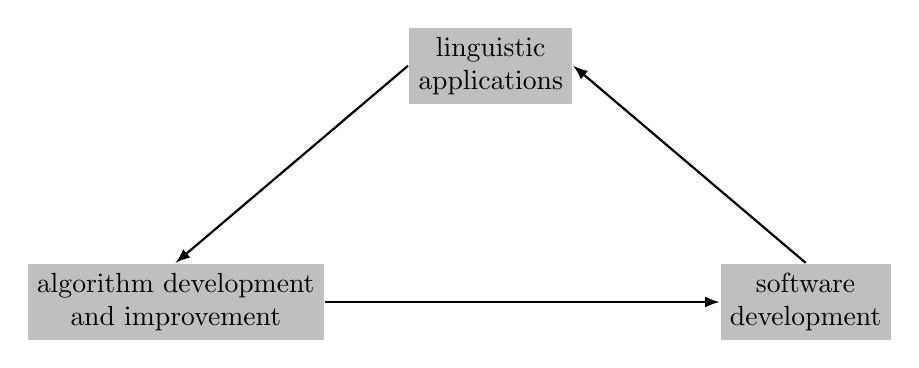
\begin{tikzpicture}
\tikzstyle{every path}=[-latex,thick]
%
\node[align=center, fill=gray!50!white] at (0,3) (L) {{linguistic} \\ {applications}};
\node[align=center, fill=gray!50!white] at (-4,0)(A) {{algorithm development} \\ {and improvement}};
\node[align=center, fill=gray!50!white] at (4,0) (C) {{software} \\ {development}};
%
\draw (L.west) -- (A.north);
\draw (A.east) -- (C.west);
\draw (C.north) -- (L.east);
\end{tikzpicture}
\caption{Exchange of ideas and innovations among applications of the subregular approach.}
\label{finaltriangle}
\end{figure}



\subsection{Linguistic applications}


The availability of subregular tools allows making progress in linguistic applications of subregular proposals.
So, for instance, one could evaluate subregular proposals in a tool-assisted way, using the encoded or automatically learned subregular models.
Subregular learning experiments, in turn, can yield important theoretical results, and highlight the improvements that can be made to the subregular algorithms or software.




\paragraph{Evaluating the subregular proposals}
One of the applications of the subregular tools is to test ideas that are available in the literature, therefore evaluating the existent subregular proposals.
So, for example, if a TSL model is proposed for a certain phenomenon, tools allow to automatically test if the TSL hypothesis is indeed consistent with the data.
Alternatively, if literature claims that some phenomenon is subsequential, it is important to verify that current implementations of the learners are indeed capable of discovering that pattern.
In such a way, implemented learners and scanners allow to verify claims made in the literature, and at the same time see the further improvements that can be made.

\paragraph{Not learning the impossible}
If an upper bound is proposed on the complexity of linguistic patterns, it is important to understand if there are any exceptions to the rule.
One of the ways to do so is to attempt learning those unattested patterns using the available subregular models,
Additionally, it is also important to research why the unattested patterns are impossible: due to the non-learnable nature of those patterns, as \cite{Lai15} suggests, or because of the unlikelihood of such a system evolving \citep{Blevins2004}.
Knowing \emph{what} patterns are not possible and \emph{why} helps to get closer to understanding the core nature of linguistic dependencies, and it, in turn, helps us to form requirements for learning algorithms extracting natural language patterns.

\paragraph{Learning experiments from data}
Finally, it is crucially important to know if the proposed subregular learners are capable of learning the target patterns of the corresponding complexity from data.
The data can be of different degrees of abstractness, ranging from the artificially generated sample with the minimal possible alphabet to raw natural language data.
Different types of linguistic phenomena need to be targeted so that we can better understand which classes and learners should be used in which case.
In my thesis, I only evaluated the behavior of learners using datasets exhibiting local dependencies, harmonies with or without blocking, and some other patterns.
Other possible target phenomena include epenthesis, deletion, metathesis, different types of dissimilations, and a variety of suprasegmental patterns.
Additionally, learning from data allows to explore the performance of the subregular learners under circumstances such as the increased size of the alphabet, the sparsity of the natural language data, or the small/large size of the training sample.
Conducting such learning experiments helps not only to evaluate the practical aspects of theoretical advancements but also to assess the performance of subregular learners on real data.

\bigskip\bigskip

Critically evaluating linguistic ideas and new findings helps to detect the improvements that need to be implemented in the subregular learning algorithms and models.
So, for example, linguists were for decades advocating for the importance of features and natural classes.
In turn, subregular algorithms would greatly benefit from a way to represent data in a less sparse way, therefore simplifying the learning.
In such a way, insights from linguistics help to highlight which algorithms need to be developed in the future, and how to improve the existent learners.




\subsection{Algorithm development and improvement}

Linguistics and applications to language patterns help to see the potential improvements of the subregular learning paradigm.
Typological work uncovers new types of dependencies and that, in turn, inspires the definition of new subregular language classes and the corresponding learners.
Old learners can be improved as well, for example, by adding linguistic features, probabilities, or combining powers of several learners.


\paragraph{Designing new algorithms}
Apart from the discussed SL, SP, TSL, and MTSL subregular languages, there are other subregular classes that capture long-distance linguistic dependencies in other ways.
Among them, there is an extension of TSL languages with the tier projection function that is sensitive to the local context (input-TSL, or ITSL), and several other classes such as MITSL, OTSL, IOTSL, and IBSP \citep{Graf17Phonology,DeSantoGraf19FG}.
Additionally, one could extend the $2$-MTSL learner from $2$ to $k$, or make sure that the learner always induces the minimal number of tiers.
Other ideas for the design of the learning algorithms are listed in section 4.3 and could be explored as well.
Additionally, the topic of adding more ``naturalness'' to the learning algorithms needs to be further explored, such as learning the feature systems of the language or finding a way to encode linguistic notions such as natural classes.


\paragraph{Implementing linguistic notions}
As mentioned in the previous subsection, the subregular learners could greatly benefit from implementing linguistic notions such as features or natural classes.
It would allow seeing the behavior of elements of the alphabet as \emph{groups} sharing some feature, instead of the current independent treatment of every segment.
Potentially, this could improve the performance of the subregular learners on natural language data.
The first steps towards incorporating features and natural classes into subregular models are taken by \cite{Strother-Garcia-HeinzEtAl-2016-UMTGICSP} and \cite{chandlee-etal-2019-learning}, and show promising results.
In the future, this line of research needs to be expanded as well.
 


\paragraph{Implementing probabilities}

Another way to improve the performance of the subregular algorithms is to add probabilities to the models.
Probabilistic modeling would allow to recognize harmony patterns even when the disharmonic words are present.
Some theoretical research is already done in this direction by \cite{HeinzRogers2010SPdist} and \cite{Shibata-Heinz-2019-MLEFRDSL}.
Also, probabilistic modeling can be combined with the feature-based and natural class-based approaches \citep{Heinz-Koirala-2010-MLEFD,VuZehfrooshEtal2018-SRLUSM}.

\paragraph{Combining the learners}
Sometimes, a target language is at the intersection of different string-based subregular languages.
For example, it can exhibit tone plateauing (SP) together with a long-distance harmony with blocking (TSL).
To learn this patter, the SP and TSL learning algorithms can be run in parallel, and the intersection of the obtained languages yields the target language \citep{Heinz10ldp,HeinzIdsardi13}.
In case of learning complex rewrite rules, further research is required since it is not clear if transformations can be combined in a way that would preserve properties such as subsequentiality.%
\footnote{Although this is an open question, research groups at Stony Brook University, University of Ottawa, and UC San Diego are currently working on it.}

\bigskip\bigskip

The availability of new ideas and algorithms in the literature gives a way of implementing them in practice.
Researchers can access the needed tools without the need to implement them from scratch if toolkits such as \emph{SigmaPie} are available and up-to-date.
Since the subregular languages and learners are closely interconnected and rely on the same basis of assumptions, the modularity of such a toolkit allows integrating new classes and learners easily.
This is an essential step for keeping a mutually beneficial exchange between the theory and the practice.


\subsection{Software development}

Some algorithms are proposed in the literature but are not yet available in the form of tools or software.
Bridging this gap helps to fast-forward the applications of the subregular models in linguistics, which, in turn, discovers the possible ways to improve those subregular algorithms.


\paragraph{Implementation of algorithms}
Some of the subregular learning algorithms are not yet implemented and therefore their practical applications are not explored.
Among them, there are the learning algorithms ISLFLA and OSLFIA which extract two subclasses of subsequential mappings that are especially useful for local phonological processes \citep{ChandleeEtAl2014,ChandleeEtAl2015}.
A learner for the class of Output $2$-TSL functions is available in \citep{BurnessMcMullin2019} and needs to be implemented as well.
\cite{chandlee-etal-2019-learning} also proposes a transduction learner for feature-based representations learning long-distance dependencies.

\paragraph{Software correctness}
To confirm the correctness of software, it is important to not rely on a single implementation.
For every subregular algorithm, there need to be several different independent implementations.
Also, some algorithms, such as OSTIA, are presented in the literature using several different pseudocodes implementing the same idea, and all those versions need to be implemented as well.
Additionally, the speed of the original implementations could be increased as well, by decreasing the big $\mathcal{O}$ complexity of the algorithm or by implementing memory-efficient techniques such as caching.

\bigskip\bigskip

Implementing the subregular learners and other functionality like scanners or sample generators helps to provide tools to linguistics, which, in its turn, can yield new results, or confirm old results using the newly available learners or models.
Also, the availability of the tools makes subregular projects easier to be approached by a beginner's level linguists, such as undergraduate researchers.

During the last decade, the field of subregular research grew in its popularity, with theoretical advancements showing that it could be used for modeling different phonological, morphological, and even syntactic patterns.
\emph{SigmaPie} \href{https://pypi.org/project/SigmaPie/}{\faCube} is the first toolkit directed towards the development of subregular tools.
It allows evaluating subregular proposals over data sets of various degree of abstractness.
In my dissertation, I showed that \emph{SigmaPie} can be used to yield new results the are relevant for theoretical and computational linguistics.
These results, in turn, can bring insights into understanding the nature of human language.
